\documentclass{ximera}

\title{Exam 1 Review}
\author{Rachel Bailey}
\license{CC: 0}         % replace with an appropriate license, or set it in xmPreamble

\begin{document}
\begin{abstract}
   This review covers covers sections...
\end{abstract}
\maketitle




\begin{problem}
Find the domains of the following functions and write them in interval notation.
\begin{enumerate}
\item $\displaystyle\frac{\ln(x-2)}{x^2-6x-7}=\begin{prompt}\answer{(2,7)}\end{prompt}\cup \answer{(7,\infty)}$
\item $\displaystyle\frac{x^2+1}{\sqrt{3x-1}}=\answer{(1/3, \infty)}$
\item $\ln(x^2-3x-4)=\answer{(-\infty, -1)}\cup \answer{(4,\infty)}$
\end{enumerate}

\end{problem}

\begin{question}
 Solve the following equations for $x$. If there are multiple solutions, list them as a comma-separated list.
\begin{enumerate}
\item $ e^{x^2+3x-17}=e$
\[
         \answer[validator=multiAns]{[-6,3]},\answer[validator=multiAns]{[-6,3]}
        \]


\item $\ln\left( \frac{1}{x}\right)=2$
\[
x=\answer{e^{-2}}
\]
\item $ 4\sin^2(x)-3=0, \quad 0\leq x\leq 2\pi$\\
\begin{selectAll}
                \choice[correct]{$\frac{\pi}{3}$}
                \choice[correct]{$\frac{2\pi}{3}$}
                \choice{$\pi$}
                \choice[correct]{$\frac{4\pi}{3}$}
                \choice[correct]{$\frac{5\pi}{3}$}
                \choice{$2\pi$}
            \end{selectAll}

\item $\ln(x+6)+\ln(x+1)=\ln(3)+2\ln(2\sqrt{x})$
\[
    x=\answer[validator=multiAns]{[2,3]},\answer[validator=multiAns]{[2,3]}
        \]


\end{enumerate}
\end{question}

\begin{problem}
Let $f(x)=\displaystyle \frac{x}{x+1}$ and $g(x)=2x^3-1$. Compute the following:
\begin{enumerate}
    \item $(f\circ g)(x)=\answer{\frac{2x^3-1}{2x^3}}$
\item $(g\circ f)(x)=\answer{\frac{2x^3}{(x+1)^3}-1}$
\item $(f\circ f)(x)=\answer{\frac{x}{2x+1}}$
\item $(g\circ g)(x)=\answer{2(2x^3-1)^3-1}$
\end{enumerate}
\end{problem}

\begin{problem}
Compute the following
\begin{enumerate}
    \item $\displaystyle\sin\left(\frac{7\pi}{4}\right)=\answer{\frac{-\sqrt{2}}{2}}$
\item $\displaystyle\tan\left(-\frac{5\pi}{3}\right)=\answer{\sqrt{3}}$
\item $\displaystyle\cos\left(\frac{13\pi}{6}\right)=\answer{\frac{\sqrt{3}}{2}}$

\end{enumerate}
\end{problem}

\begin{problem}
    Find and simplify the \textit{difference quotient} $\frac{f(a+h)-f(a)}{h}$ for the following functions.
    \begin{enumerate}
        \item $f(x)=3x^2-1 =\answer{6a+3h}$
        \item $f(x)=\frac{1}{x+1}=\answer{-\frac{1}{(a+1)(a+h+1)}}$
    \end{enumerate}
\end{problem}

\begin{problem}
Determine the method needed for the following limit and then compute the limit. If they do not exist, write DNE.
\begin{enumerate}
    \item $\displaystyle \lim\limits_{x\to -3}\frac{x^2-x-12}{x+3}$\\
   Method: \wordChoice{
                \choice[correct]{factoring}
                \choice{multiply by conjugate}
                \choice{common denominator}
                \choice{direct substitution}
                \choice{c/0 type}
                \choice{squeeze theorem}
                }
    \[ \lim\limits_{x\to -3}\frac{x^2-x-12}{x+3}=\answer{-7}
    \]

    \item $\displaystyle \lim\limits_{x\to 0}\frac{x^4-4x^2+34}{x-17}$\\
     Method: \wordChoice{
                \choice{factoring}
                \choice{multiply by conjugate}
                \choice{common denominator}
                \choice[correct]{direct substitution}
                \choice{c/0 type}
                \choice{squeeze theorem}
                }
              
               \[ \lim\limits_{x\to 0}\frac{x^4-4x^2+34}{x-17}=\answer{-2}
    \]
 
 \item $\displaystyle \lim\limits_{x\to 4^-}\frac{3-x}{4-x}$\\
   Method: \wordChoice{
                \choice{factoring}
                \choice{multiply by conjugate}
                \choice{common denominator}
                \choice{direct substitution}
                \choice[correct]{c/0 type}
                \choice{squeeze theorem}
                }
     \[ \lim\limits_{x\to 4^-}\frac{3-x}{4-x}=\answer{-\infty}
    \]
 

    \item $\displaystyle \lim\limits_{x\to 4^+}\frac{3-x}{4-x}$\\
     Method: \wordChoice{
                \choice{factoring}
                \choice{multiply by conjugate}
                \choice{common denominator}
                \choice{direct substitution}
                \choice[correct]{c/0 type}
                \choice{squeeze theorem}
                }
    \[\lim\limits_{x\to 4^+}\frac{3-x}{4-x}=\answer{+\infty}
    \]
 

    \item $\displaystyle \lim\limits_{x\to 3}\frac{\frac{1}{x}-\frac{1}{3}}{x-3}$\\
   Method: \wordChoice{
                \choice{factoring}
                \choice{multiply by conjugate}
                \choice[correct]{common denominator}
                \choice{direct substitution}
                \choice{c/0 type}
                \choice{squeeze theorem}
                }
            
    \[\lim\limits_{x\to 3}\frac{\frac{1}{x}-\frac{1}{3}}{x-3}=\answer{-\frac{1}{9}}
    \]
 

    \item $\displaystyle\lim\limits_{x\to 0}\frac{\sqrt{2+x}-\sqrt{2}}{x}$\\
     Method: \wordChoice{
                \choice{factoring}
                \choice[correct]{multiply by conjugate}
                \choice{common denominator}
                \choice{direct substitution}
                \choice{c/0 type}
                \choice{squeeze theorem}
                }
    \[\lim\limits_{x\to 0}\frac{\sqrt{2+x}-\sqrt{2}}{x}=\answer{\frac{1}{2\sqrt{2}}}
    \]

\item $\displaystyle \lim\limits_{x\to \infty}\frac{\sin^2(x)}{\sqrt{x}}$\\
 Method: \wordChoice{
                \choice{factoring}
                \choice{multiply by conjugate}
                \choice{common denominator}
                \choice{direct substitution}
                \choice{c/0 type}
                \choice[correct]{squeeze theorem}
                }
     \[ \lim\limits_{x\to \infty}\frac{\sin^2(x)}{\sqrt{x}}=\answer{0}
                 \]
   
\item $\displaystyle  \lim\limits_{x\to \infty}\frac{12+e^x}{4-2e^x}$\\
  Method: \wordChoice{
                \choice[correct]{factoring}
                \choice{multiply by conjugate}
                \choice{common denominator}
                \choice{direct substitution}
                \choice{c/0 type}
                }
    \[\lim\limits_{x\to \infty}\frac{12+e^x}{4-2e^x}=\answer{-\frac{1}{2}}
    \]


\item $\displaystyle \lim\limits_{x\to \infty}\frac{x}{\sqrt{9x^2+x}+3x}$\\
 Method: \wordChoice{
                \choice{factoring}
                \choice{multiply by conjugate}
                \choice{common denominator}
                \choice{direct substitution}
                \choice{c/0 type}
                \choice[correct]{multiply by $1/x^p$}
                }
    \[\lim\limits_{x\to \infty}\frac{x}{\sqrt{9x^2+x}+3x}=\answer{\frac{1}{6}}
    \]


\item $\displaystyle \lim\limits_{x\to -\infty}\frac{3x^2+x}{4x^3-2x+1}$\\

 Method: \wordChoice{
                \choice{factoring}
                \choice{multiply by conjugate}
                \choice{common denominator}
                \choice{direct substitution}
                \choice{c/0 type}
                \choice[correct]{mulitply by $1/x^p$}
                }
\[\lim\limits_{x\to -\infty}\frac{3x^2+x}{4x^3-2x+1}=\answer{0}
                \]

\end{enumerate}
\end{problem}


\begin{problem}
 
Let \[f(x)=\frac{x^2-x-2}{x^2-2x}
\] 
\begin{enumerate}
\item What is the domain of $f(x)$? Write your answer in interval notation.
\[
\answer{(-\infty,0)\cup (0,2)\cup(2, \infty)}
\]
\item  List any vertical or horizontal asymptotes and/or holes of the graph of $f(x)$. Be sure to justify your answer!
\[
\text{vertical: } x=\answer{0}
\]
\[
\text{horizontal: } y=\answer{1}
\]
\[
\text{holes at: } x=\answer{2}
\]

\item Compute $\lim\limits_{x\to 2}f(x).$
\[
\lim\limits_{x\to 2}f(x)=\answer{\frac{3}{2}}
\]
\item How could we define $f(2)$ so that $f(x)$ is continuous at $x=2$?\\
\\

For $f(x)$ to be continuous at $x=2$, we need $\lim\limits_{x\to 2}f(x)=f(\answer{2})$, thus, if we can define $f(2)=\answer{\frac{3}{2}}$, $f(x)$ will be continuous at $x=2$.


\end{enumerate}
\end{problem}

\begin{problem}
Consider the graph of $f(x)$ below.
\begin{image}
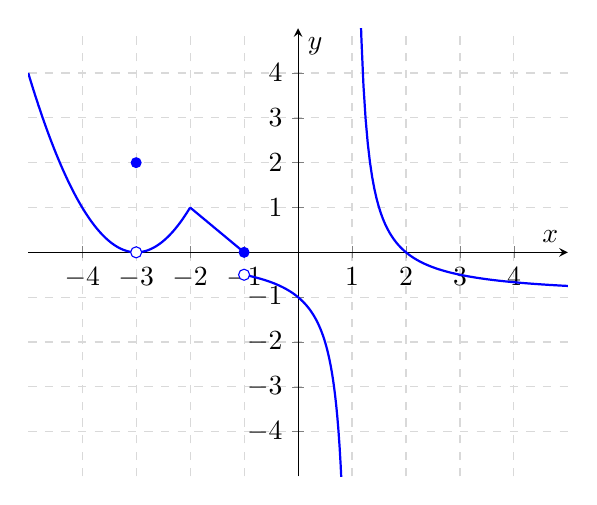
\begin{tikzpicture}
\begin{axis}[
    axis lines = center,
    xlabel = {$x$},
    ylabel = {$y$},
    xmin = -5, xmax = 5,
    ymin = -5, ymax = 5,
    samples = 100,
     xtick = {-4,...,4},
    ytick = {-4,...,4},
    grid = both,
    grid style = {dashed, gray!30},
]
    % First piece: x^2 for x <= 0
    \addplot[domain=-5:-2, thick, blue] {(x+3)^2};
    
    % Second piece: x + 2 for x > 0
    \addplot[domain=-2:-1, thick, blue] {-x-1};

     \addplot[domain=-1:0.99, thick, blue] {(x)/(x-1)-1};

      \addplot[domain=1.01:5, thick, blue] {(2-x)/(x-1)};
    
    % Endpoints (solid or hollow circles)
    \fill[blue] (axis cs:-3,2) circle (2pt); % Included endpoint at (0,0)
    \draw[blue, fill=white] (axis cs:-3,0) circle (2pt); % Excluded endpoint at (0,2)
\fill[blue] (axis cs:-1,0) circle (2pt); % Included endpoint at (0,0)
\draw[blue, fill=white] (axis cs:-1,-1/2) circle (2pt); 


\end{axis}
\end{tikzpicture}
\end{image}
%\begin{center}
%
\includegraphics[scale=0.35]{xmPictures/Exam1PracticeGraph.pdf}
%\end{center}

\begin{enumerate}
    \item State all the discontinuities of $f(x)$ and list their types.\\
    
    $x=\answer{-3}$ is a \wordChoice{
                \choice[correct]{hole}
                \choice{jump discontinuity}
                \choice{vertical asymptote}
                }, \\
    $x=\answer{-2}$ is a \wordChoice{
                \choice[correct]{hole}
                \choice{jump discontinuity}
                \choice{vertical asymptote}
                }, \\
    $x=\answer{-1}$ is a \wordChoice{
                \choice{hole}
                \choice[correct]{jump discontinuity}
                \choice{vertical asymptote}
                }, \\
    $x=\answer{1}$ is a \wordChoice{
                \choice{hole}
                \choice{jump discontinuity}
                \choice[correct]{vertical asymptote}
                }
   

    \item Find the following:

    \begin{enumerate}
        \item $\lim\limits_{x\to 0}f(x)=\begin{prompt}
            \answer{-1}
        \end{prompt}$
  
        \item $\lim\limits_{x\to -1^-}f(x)=\begin{prompt}
            \answer{0}
        \end{prompt}$
     
        \item $\lim\limits_{x\to -1^+}f(x)=\begin{prompt}
            \answer{-\frac{1}{2}}
        \end{prompt}$
  
        \item $\lim\limits_{x\to -1}f(x)=\begin{prompt}
            \answer{DNE}
        \end{prompt}$

        \item $\lim\limits_{x\to -3^-}f(x)=\begin{prompt}
            \answer{0}
        \end{prompt}$

        \item $\lim\limits_{x\to -3^+}f(x)=\begin{prompt}
            \answer{0}
        \end{prompt}$
      
          \item $\lim\limits_{x\to -3}f(x)=\begin{prompt}
            \answer{0}
        \end{prompt}$
     
        \item $\lim\limits_{x\to 1^+}f(x)=\begin{prompt}
            \answer{\infty}
        \end{prompt}$
    
        \item $\lim\limits_{x\to 1^-}f(x)=\begin{prompt}
            \answer{-\infty}
        \end{prompt}$
 
        \item $f(-3)=\begin{prompt}
            \answer{2}
        \end{prompt}$

        \item $f(1)=\begin{prompt}
    \answer{DNE}
        \end{prompt}$

    \item $\lim\limits_{x\to \infty}f(x)=\begin{prompt}
            \answer{-1}
        \end{prompt}$

    \item $\lim\limits_{x\to -\infty}f(x)=\begin{prompt}
            \answer{\infty}
        \end{prompt}$
           \end{enumerate}

\end{enumerate}


\end{problem}







\end{document}
